% id: 162-10
% book: 100발100중 3-1 기말 · 01 3-1 기말(이차방정식·이차함수·부록)
% section: 파이널 모의고사 5회
% figure: crop:fig-162-10.png
% answer: ③
% answer_source: 답지(빠른정답)
% variant_level: 0 (원본 전사)
% 이 파일은 build.mjs 가 items.json 에서 만든다. 고칠 때는 items.json 을 고친다.
\smash{\raisebox{1.5mm}{\dmkichul{100발100중 3-1 기말 162쪽 10번}}}
\noindent\begin{minipage}[t]{0.58\linewidth}\vspace{0pt}\raggedright 그림과 같이 가로의 길이가 $16\mkern3mu \mathrm{cm}$, 세로의 길이가 $10\mkern3mu \mathrm{cm}$인 직사각형 $\pt{ABCD}$가 있다. 가로의 길이는 매초 $2\mkern3mu \mathrm{cm}$씩 줄어들고, 세로의 길이는 매초 $1\mkern3mu \mathrm{cm}$씩 늘어날 때, 넓이가 $90\mkern3mu \mathrm{cm}^2$가 되는 데 걸리는 시간은? \mbox{[4점]}\end{minipage}\hfill\begin{minipage}[t]{0.4\linewidth}\vspace{0pt}\centering 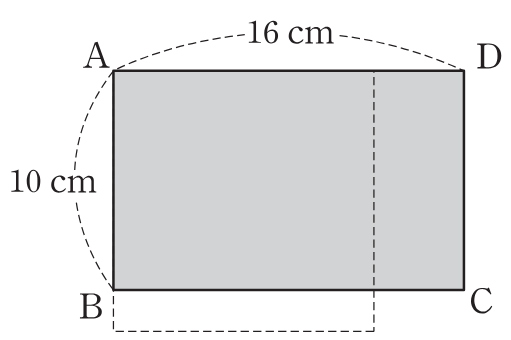
\includegraphics[width=122.5pt]{figures/fig-162-10.png}\end{minipage}\par
\begin{choices32}{$2$초}{$3$초}{$5$초}{$7$초}{$9$초}\end{choices32}
